\documentclass[fleqn]{beamer}

\usepackage[british]{babel}
\usepackage{graphicx,ru,url}
\graphicspath{{../tex/figures/}}
\usepackage{amsmath}
% Use Times for math font and text font.
\RequirePackage[T1]{fontenc}
%\RequirePackage{txfonts}
% bold math must be loaded after Times font
\usepackage{bm}
\usepackage{booktabs} % nice rules (thick lines) for tables
\usepackage{microtype} % improves typography for PDF
\usepackage{xcolor} % Allows colors in fonts

\usepackage{tikz} % Allows creation of tikz pictures
\usetikzlibrary{arrows}
\usetikzlibrary{arrows.meta}

\usepackage{verbatim}
\usetikzlibrary{arrows,shapes,snakes}
\usetikzlibrary{patterns}
\usepackage{url}
\usepackage{ifthen}
\usepackage{subcaption}
\usepackage{slashbox} % backslashbox in a table

% typesetting using the algorithmicx package
% detail at: https://en.wikibooks.org/wiki/LaTeX/Algorithms and https://tex.stackexchange.com/questions/229355/algorithm-algorithmic-algorithmicx-algorithm2e-algpseudocode-confused
\usepackage{algorithm}
\usepackage{algpseudocode}

\usepackage{multibib}
\newcites{Mypub}{List of Publications}

% The title of the presentation:
%  - first a short version which is visible at the bottom of each slide;
%  - second the full title shown on the title slide;
\title[KSU Beam Characterization]{Neutron Flux Characterization of the Kansas State University TRIGA Mark II's Northeast Beam Port}

% Optional: a subtitle to be displayed on the title slide
%\subtitle{Show where you're from}

% The author(s) of the presentation:
%  - again first a short version to be displayed at the bottom;
%  - next the full list of authors, which may include contact information;
\author[John Boyington]{
    John Boyington\\
    Advisor: Prof.~Jeremy Roberts}

% The institute:
%  - to start the name of the university as displayed on the top of each slide
%    this can be adjusted such that you can also create a Dutch version
%  - next the institute information as displayed on the title slide
\institute[Kansas State University]{
    Department of Mechanical and Nuclear Engineering \\
    Kansas State University}

% Add a date and possibly the name of the event to the slides
%  - again first a short version to be shown at the bottom of each slide
%  - second the full date and event name for the title slide
\date[Master's Defense]{
    Master's Defense\\
    Ward Hall 135\\
    August 12, 2019}

\begin{document}
% These two commands allow bonus slides at the end
% The bonus slides will not be numbered
\newcommand{\beginbackup}{
    \newcounter{framenumbervorappendix}
    \setcounter{framenumbervorappendix}{\value{framenumber}}
}
\newcommand{\backupend}{
    \addtocounter{framenumbervorappendix}{-\value{framenumber}}
    \addtocounter{framenumber}{\value{framenumbervorappendix}}
}


%%% Introduction (2) ---------------------------------------------------------------------------------------
%%%%%%%%%%%%%%%%%%%% title slide

\begin{frame}
\titlepage
\end{frame}

%%%%%%%%%%%%%%%%%%%% presentation outline
\begin{frame}
\frametitle{Outline}
\begin{itemize}
\item Neutron Spectrometry and Deconvolution
\item Simulated Work
\item Experimental Work
\item Conclusions and Future Work
\end{itemize}
\end{frame}

%%% Lit Review Stuff (6) ---------------------------------------------------------------------------------------
\section{Neutron Spectrometry and Deconvolution}
%%%%%%%%%%%%%%%%%%%%% bonner sphere spectrometers
\begin{frame}
\frametitle{Bonner Sphere Spectrometers}
\begin{columns}[c]
\begin{column}{.5\textwidth}
\begin{figure}
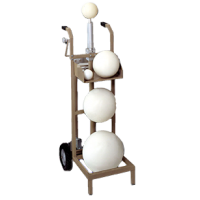
\includegraphics[width=\textwidth]{bss}
\caption{Bonner Sphere Spectrometer}
\end{figure}
\end{column}
\begin{column}{.5\textwidth}
Text\\
Text\\
Text\\
\end{column}
\end{columns}
\end{frame}

%%%%%%%%%%%%%%%%%%%%% gold foil based spectrometers
\begin{frame}
\frametitle{Foil-based Spectrometers}

Text here about gold foil spectrometers.

\end{frame}

%%%%%%%%%%%%%%%%%%%%% the mathematic formulation/unfolding
\begin{frame}
\frametitle{Problem Formulation}
\begin{equation}
\label{eqn:disc-response}
N_k + \epsilon_k = \sum_i R_{ki} \phi_i, \quad k = 1,\ldots, m .
\end{equation}
\end{frame}


%%%%%%%%%%%%%%%%%%%%% doroshenko directed divergence
\begin{frame}
\frametitle{Doroshenko Directed Divergence}

\begin{equation}
\label{eqn:doroshenko}
\phi_j^{k + 1} = \phi_j^{k} (\frac{\sum_i \frac{R_{ji}}{\sum_j R_{ij} \phi_j^k}}{\sum_i \frac{R_{ji}}{N_i}}) 
\end{equation}

\end{frame}

%%%%%%%%%%%%%%%%%%%%% gravel/sandii
\begin{frame}
\frametitle{Gravel}

\begin{equation}
\label{eqn:sandii}
\phi_j^{k + 1} = \phi_j^{k} exp(\frac{\sum_i W_{ji}^k \log(\frac{N_i}{\sum_{j'} R_{ij'} \phi_{j'}^k})}{\sum_i W_{ji}^k}) ,
\end{equation}

\begin{equation}
\label{eqn:gravel-w}
W_{ji}^k = \frac{R_{ij} \phi_{j}^k}{\sum_{j'} R_{ij'} \phi_{j'}^k} \frac{N_i^2}{\sigma_i^2} ,
\end{equation}
\end{frame}

%%%%%%%%%%%%%%%%%%%%% maxed
\begin{frame}
\frametitle{MAXED}
\begin{equation}
\label{eqn:maxed-skilling}
S = - \sum [\phi_j \ln (\frac{\phi_j}{\phi_j^{DEF}}) + \phi_j^{DEF} - \phi_j]
\end{equation}
\end{frame}


%%% NEBP Modeling Effort (10) ---------------------------------------------------------------------------------------
\section{Simulated Work}
%%%%%%%%%%%%%%%%%%%%% modeling steps/overview
\begin{frame}
\frametitle{Modeling Overview}

\end{frame}

%%%%%%%%%%%%%%%%%%%%% existing model
\begin{frame}
\frametitle{Existing Model}

\end{frame}

%%%%%%%%%%%%%%%%%%%%% nebp additions
\begin{frame}
\frametitle{NEBP Additions}

\end{frame}

%%%%%%%%%%%%%%%%%%%%% fission tally results I
\begin{frame}
\frametitle{Fission Tally Results}

\end{frame}

%%%%%%%%%%%%%%%%%%%%% fission tally results II
\begin{frame}
\frametitle{Fission Tally Results}

\end{frame}

%%%%%%%%%%%%%%%%%%%%% applyting advantg
\begin{frame}
\frametitle{Applying ADVANTG}

\end{frame}

%%%%%%%%%%%%%%%%%%%%% notes on speedup/runtime/cores,etc.
\begin{frame}
\frametitle{Runtime, speedup, etc.}

\end{frame}

%%%%%%%%%%%%%%%%%%%%% energy distribution
\begin{frame}
\frametitle{Spectral Flux}

\end{frame}

%%%%%%%%%%%%%%%%%%%%% cosine distribution
\begin{frame}
\frametitle{Angular Flux}

\end{frame}

%%%%%%%%%%%%%%%%%%%%% radial distribution
\begin{frame}
\frametitle{Radial Flux}

\end{frame}

%%% NEBP Experimental Campaign (14) ---------------------------------------------------------------------------------------
\section{Experimental Work}
%%%%%%%%%%%%%%%%%%%%% modeling steps
\begin{frame}
\frametitle{Response Function Generation}

\end{frame}

%%%%%%%%%%%%%%%%%%%%% foil tube response functions
\begin{frame}
\frametitle{Foil Tube Response Functions}

\end{frame}

%%%%%%%%%%%%%%%%%%%%% bonner sphere response functions
\begin{frame}
\frametitle{Bonner Sphere Response Functions}

\end{frame}

%%%%%%%%%%%%%%%%%%%%% experimental procedures: ft
\begin{frame}
\frametitle{Foil Tube Experimental Procedures}

\end{frame}

%%%%%%%%%%%%%%%%%%%%% experimental procedures: bss
\begin{frame}
\frametitle{Bonner Sphere Spectrometer Experimental Procedures}

\end{frame}

%%%%%%%%%%%%%%%%%%%%% gold foil post processing
\begin{frame}
\frametitle{Foil Tube Postprocessing}

\end{frame}

%%%%%%%%%%%%%%%%%%%%% transient mathematics
\begin{frame}
\frametitle{Capturing Flux Transients}

\end{frame}

\begin{frame}
\frametitle{Capturing Flux Transients cont.}

\end{frame}

%%%%%%%%%%%%%%%%%%%%% bss postprocessing
\begin{frame}
\frametitle{Bonner Sphere Postprocessing}

\end{frame}

%%%%%%%%%%%%%%%%%%%%% response comparison: ft
\begin{frame}
\frametitle{Response Comparison: Foil Tube}

\end{frame}

%%%%%%%%%%%%%%%%%%%%% response comparison: bss
\begin{frame}
\frametitle{Response Comparison: Bonner Sphere}

\end{frame}

%%%%%%%%%%%%%%%%%%%%% spectral unfolding: parameters
\begin{frame}
\frametitle{Spectral Unfolding Parameters}

\end{frame}

%%%%%%%%%%%%%%%%%%%%% spectral unfolding: doroshenko
\begin{frame}
\frametitle{Spectral Unfolding: Doroshenko Directed Divergence}

\end{frame}

%%%%%%%%%%%%%%%%%%%%% spectral unfolding: gravel
\begin{frame}
\frametitle{Spectral Unfolding: Gravel}

\end{frame}

%%%%%%%%%%%%%%%%%%%%% spectral unfolding: maxed
\begin{frame}
\frametitle{Spectral Unfolding MAXED}

\end{frame}

%%% Conclusions & Future Work (3) ---------------------------------------------------------------------------------------
\section{Conclusions and Future Work}
%%%%%%%%%%%%%%%%%%%%% conclusions
\begin{frame}
\frametitle{Conclusions}

\end{frame}

%%%%%%%%%%%%%%%%%%%%% future work
\begin{frame}
\frametitle{Future Work}

\end{frame}

%%%%%%%%%%%%%%%%%%%%% references
\begin{frame}
\frametitle{References}

\end{frame}




\end{document}



